%\subsection{Het gebruik van de LED matrix.}
\chapter{Het gebruik van de LED matrix \normalsize{(week 4)}.}
\label{chap:matrix}

Indien we een externe LED op de microbit aansluiten, zoals in figuur \ref{fig:schemaExLd} wordt weergegeven, kunnen we deze direct aansturen, zoals listing \ref{lst:extLd} laat zien.
\begin{figure}[h!]
	
	\centering
	\begin{center} 	
		\begin{subfigure}[b]{0.43\textwidth}
			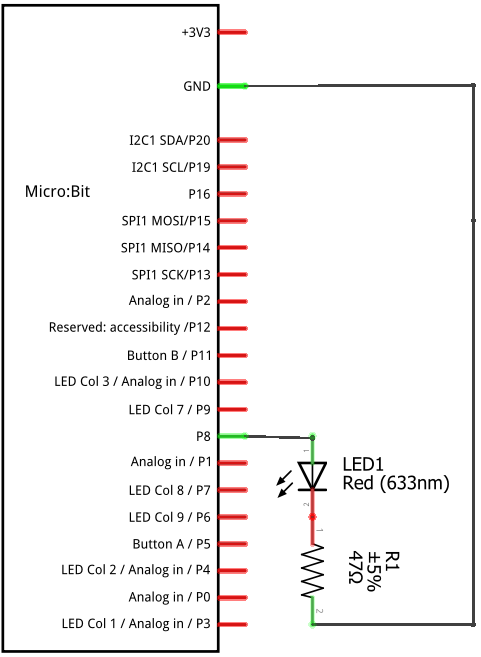
\includegraphics[width=0.85\textwidth]{figuren/externeLedCr}
			\caption{Een externe led aangesloten op P08 }
			\label{fig:schemaExLd}
			
		\end{subfigure}
		\begin{subfigure}[b]{0.46\textwidth}
\begin{lstlisting}[caption={Het aansturen van een externe LED.},label={lst:extLd}]
const int externeLed = 8;
				
   void setup() {

		pinMode(externeLed, OUTPUT);  
	}
				
	void loop() {
		digitalWrite(externeLed,HIGH);
		delay(500);
		digitalWrite(externeLed,LOW);
		delay(500); 
	}
\end{lstlisting}
		\end{subfigure}
		\captionsetup{justification=centering}
		\caption{Het aansturen van een externe LED. }
		\label{fig:exampleInh}
	\end{center}	
\end{figure}
De externe LED wordt aangesloten op poortnummer 8. In de \textcolor{arduinoGreen}{setup}() wordt dit poortnummer op output gezet. 
In de \textcolor{arduinoGreen}{loop}() wordt als eerste een spanning gezet op poort 8 (\textcolor{arduinoOrange}{digitalWrite}(externeLed, \textcolor{arduinoBlue}{HIGH});) waardoor een elektrische stroom door de LED gaat lopen en deze licht gaat geven. 
Hierna wordt een halve seconde gewacht, daarna wordt op poort 8,  0 Volt gezet (\textcolor{arduinoOrange}{digitalWrite}(externeLed, \textcolor{arduinoBlue}{LOW});) en gaat de LED uit (er loopt geen elektrische stroom meer door de LED).
Kijken we naar de listings \ref{lst:blink} en \ref{lst:changeBut}, dan zien we dat er twee output poorten (4 en 21) nodig zijn om de linkerboven LED in het matrix display aan te sturen. 

\begin{minipage}{\textwidth} 
	\begin{minipage}[b]{0.49\textwidth}
		\centering
		\begin{tabular}{|c|c|} \hline
			\textbf{micro:bit} & \textbf{pinnummer} \\ \hline
			COL1	 & 4  \\  \hline
			COL2	 & 7  \\  \hline
			COL3	 & 3  \\  \hline
			COL4	 & 6  \\  \hline
			COL5	 & 10  \\  \hline
			ROW1	 & 21  \\  \hline
			ROW2	 & 22  \\  \hline
			ROW3	 & 23  \\  \hline
			ROW4	 & 24  \\  \hline
			ROW5	 & 25  \\  \hline
			
		\end{tabular}
		\captionof{table}{Microbit-matrix en de arduino pinnummers.}
	\end{minipage}
	\hfill
	\begin{minipage}[b]{0.49\textwidth}
		\centering
		%		  \includegraphics[scale=0.3]{figuren/LedMatrixV2}
		\includegraphics[width=0.7 \linewidth]{figuren/LedMatrixV2}
		\captionof{figure}{A De LEDs aansluitingen van het matrix display \cite{microbitschematicV2}.}
		\label{fig:matrix}
	\end{minipage}
\end{minipage}

Dit heeft te maken met het principe van een matrix, zoals in figuur \ref{fig:matrix} te zien is. 
Om zoals in het programma blink ( listing \ref{lst:blink}),  LED D2 (figuur \ref{fig:matrix}) licht te laten geven, zal er een elektrische stroom moeten lopen van ROW1 naar COL1. Om dit voor elkaar te krijgen moet zowel ROW1 als COL1 op output gezet worden, verder zal COL1 \textcolor{arduinoBlue}{LOW} en ROW1 \textcolor{arduinoBlue}{HIGH} gemaakt moeten worden, zoals te zien is in listing \ref{lst:linkbvn}.
\begin{lstlisting}[caption={Zet de linkerboven LED van de matrix aan},label={lst:linkbvn}]
	const int COL1 = 4;   
	const int ROW1 = 21;   
	
	void setup() {
		pinMode(COL1,OUTPUT);    //zet de port COL1 op output
		pinMode(ROW1,OUTPUT);    //zet de port ROW1 op output
		digitalWrite(COL1, LOW); //zet COL1 op 0 Volt
		digitalWrite(ROW1, HIGH);//Zet electrische spanning op ROW1  
	}
	
	void loop() {
	}
\end{lstlisting}

\textbf{Opdracht \ref{chap:matrix}A:}


Open het voorbeeldprogramma matrixLed, compileer het en upload de code naar de micro:bit. Om het programma uit te breiden zodat de LEDs op alle 4 de hoekpunten licht gaan geven, wordt:
	

	\begin{enumerate}[label=(\roman*)]
		\item De onderstaande waarheidstabel ingevuld.
		
%		\begin{table}
		%	\resizebox{\linewidth}{!}{	
%			\begin{tabular}{|c|c|c|c|c|c|c|c|c|c|c|} \hline
\scalebox{0.78} {
           $\begin{array}{|c|c|c|c|c|c|c|c|c|c|c|} \hline
				%	\rowstyle{\bfseries}%
				LED&	COL1 & COL2 &  COL3 &  COL4 &  COL5 &ROW1&ROW2&ROW3&ROW4&ROW5 \\ \hline
				D2&0&1&1&1&1&1&0&0&0&0 \\ \hline
				D10&&&&&&&&&& \\ \hline	
				..&&&&&&&&&& \\ \hline	
				..&&&&&&&&&& \\ \hline	
%				5&&&&&&&&&& \\ \hline	
				
				\end{array}	$ }
%		\end{tabular} %}
%	\end{table}
		\item De code van Listing 5.2 uitgebreid aan de hand van de waarheidstabel van opdracht a.\\
		\textbf{Upload deze opgave als opgave 5A op blackboard.}
		
	\end{enumerate}


%\newpage
\textbf{Opdracht \ref{chap:matrix}B:}

	 Zoals bekend verondersteld mag worden, werkt een computer nog steeds digitaal, oftewel een '1' of een '0'.
	Zoals uit opgave A gebleken is, is het besturen van de LEDs in de matrix een kwestie van de juiste outputlijnen \textcolor{arduinoBlue}{HIGH} of \textcolor{arduinoBlue}{LOW} maken.
	
	Bij deze opgave zetten we als eerst op de bovenste rij de waarde 1 (00001), een seconde later de bovenste rij uit en op de $2^{e}$ rij de waarde 2 (00010). Een seconde later de $2^{e}$ rij uit en op de $3^{e}$ rij de waarde 3.
	Een seconde later de $3^{e}$ rij uit en op de $4^{e}$ rij de waarde 4.
	Een seconde later de $4^{e}$ rij uit en op de $5^{e}$ rij de waarde 5.
	Daarna wordt er opnieuw begonnen.Het resultaat is te zien in figuur \ref{fig:binCount}
	

		\begin{figure}[h!]
		\begin{subfigure}[b]{0.19\textwidth}
			\includegraphics[width=.98\linewidth]{figuren/matrix/mEen}
   
		\end{subfigure}
		\begin{subfigure}[b]{0.19\textwidth}
			\includegraphics[width=.98\linewidth]{figuren/matrix/mTwee}
		\end{subfigure}		
		\begin{subfigure}[b]{0.19\textwidth}
		     \includegraphics[width=.98\linewidth]{figuren/matrix/mDrie}
	   \end{subfigure}		
      \begin{subfigure}[b]{0.19\textwidth}
             \includegraphics[width=.98\linewidth]{figuren/matrix/mVier}
       \end{subfigure}	
      \begin{subfigure}[b]{0.19\textwidth}
           \includegraphics[width=.98\linewidth]{figuren/matrix/mVijf}
       \end{subfigure}	
       \caption{Binair tellen van 1 t/m 5.}
       \label{fig:binCount}
	\end{figure}
Begin als eerste met het invullen van de onderstaande waarheidstabel:
\begin{table}[h!]
	\resizebox{\textwidth}{!}{	
	\begin{tabular}{|c|c|c|c|c|c|c|c|c|c|c|} \hline
	%	\rowstyle{\bfseries}%
	Waarde&	COL1 & COL2 &  COL3 &  COL4 &  COL5 &ROW1&ROW2&ROW3&ROW4&ROW5 \\ \hline
		1&1&1&1&1&0&1&0&0&0&0 \\ \hline
		2&&&&&&&&&& \\ \hline	
	    3&&&&&&&&&& \\ \hline	
		4&&&&&&&&&& \\ \hline	
		5&&&&&&&&&& \\ \hline		
	\end{tabular}}
\end{table}

\textbf{Upload deze opgave als opgave 5B op blackboard.}
Tip:\\
Vergeet niet de pinnen in de output mode te zetten.

